\chapter{Clustering basado en densidades: DBSCAN}\label{TEMA5}

\section{DBSCAN}

El algoritmo \textbf{DBSCAN} (\textit{Density-Based Spatial Clustering of Applications with Noise}) es una técnica de agrupamiento no supervisada que destaca por identificar clústeres de forma arbitraria en conjuntos de datos que
 contienen ruido y distribuciones no lineales.

DBSCAN trabaja identificando regiones densas de puntos y expandiéndose a partir de estos. Además, no necesita especificar el número de clústeres iniciales. Utiliza dos parámetros principales: $\epsilon$ (épsilon), que define el radio de vecindad de un punto, y MinPts, que determina el número mínimo de puntos necesarios para formar un clúster. Un punto se considera parte de un clúster si al menos MinPts puntos caen dentro de su radio $\epsilon$.  DBSCAN tiene la capacidad de identificar puntos de datos que no pertenecen a ningún clúster.

\section{Hiperparámetros}
\begin{itemize}
    \item \textbf{Épsilon} ($\epsilon$): es la distancia máxima entre dos puntos para que se consideren vecinos el uno del otro. Es decir, si la distancia entre dos puntos es menor o igual a $\epsilon$ se consideran vecinos. Si este valor es muy pequeño, una gran parte de los datos se considerarán como valor atípico.

    \item Mínimo número de puntos: el número mínimo de puntos que debe formar un grupo denso. Como regla general, los mínimos se pueden derivar del número de dimensiones D en el conjunto de datos como mínimo número de puntos >= D+1.
\end{itemize}


En este algoritmo tenemos tres tipos de puntos de datos:

\begin{itemize}
    \item  \textbf{Punto central}: es considerado punto central si tiene más puntos MinPts dentro de los eps ($\epsilon$).

    \item  \textbf{Punto fronterizo}: un punto que tiene menos de MinPts dentro de los eps ($\epsilon$), pero que está en las proximidades de un punto central.

    \item \textbf{Ruido o valor atípico}: un punto que no es un punto central o un punto fronterizo.
\end{itemize}

\section{Pasos de DBSCAN}
\begin{enumerate}
    \item Encuentra todos los puntos vecinos dentro de eps ($\epsilon$) e identifica los puntos centrales o visitados con más vecinos teniendo en cuenta el número.
    \item  Para cada punto central, si aún no le han asignado grupo, se crea un nuevo grupo.

    \item  De manera recursiva encuentra todos los puntos conectados por densidad y asígnalos al mismo grupo que el punto central. Un punto a y b están conectados por densidad si existe un punto c que tiene un número suficiente de puntos en sus vecinos y ambos puntos a y b están dentro de la distancia $\epsilon$. Es un proceso de encadenamiento; entonces, si a es vecino de c, c es vecino de d y d es vecino de e, lo que a su vez indica que d es vecino de a, además implica que b es vecino de a.

    \item Repetir con todos los puntos restantes no visitados en el conjunto de datos. Aquellos puntos que no pertenecen a ningún grupo son considerados ruido o \textit{outliers}.
\end{enumerate}

\section{Métricas de evaluación de DBSCAN}

\subsection{Índice Rand}
 Este índice mide la similitud entre dos agrupaciones (clústeres) de un conjunto de datos: una agrupación «predicha» y una agrupación de referencia que puede ser una agrupación hecha por otro algoritmo de clustering. 

Definimos las siguientes cantidades: 

\begin{itemize}
     \item a: número de pares de puntos que están en el mismo clúster en ambos agrupamientos.
     \item b: número de pares de puntos que están en clústeres diferentes en ambos agrupamientos.

     \item c: número de pares de puntos que están en el mismo clúster en el agrupamiento real, pero en clústeres diferentes en el agrupamiento predicho.

     \item d: número de pares de puntos que están en el mismo clúster en el agrupamiento predicho, pero en clústeres diferentes en el agrupamiento real.
 \end{itemize}

 El índice Rand se calcula usando la siguiente fórmula:

\begin{equation*}
    \text{Índice Rand}=\dfrac{a+b}{a+b+c+d}
\end{equation*}

Se puede interpretar de la siguiente manera: cuanto más cerca esté de $1$ indica una coincidencia perfecta entre los dos agrupamientos; un valor cercano a $0$ indica que no hay acuerdo entre los dos agrupamientos; y, un valor de 0.5, indica que la similitud entre los agrupamientos es similar a la que se esperaría al azar.


\subsection{Coeficiente de la silueta}
La puntuación de silueta mide qué tan similar es un punto a los puntos de su propio clúster (cohesión) en comparación con los puntos del clúster más cercano (separación). Se define para cada punto y luego se puede promediar para todos los puntos en el conjunto de datos.

Para cada punto $i$: calculamos la \textbf{cohesión} $a_i$ que es la distancia promedio entre el punto $i$ y todos los demás puntos en el mismo clúster; la \textbf{separación} $b_i$ la distancia promedio entre el punto i y todos los puntos en el clúster más cercano diferente del suyo.

La puntuación de silueta para el punto $i$ se define como:
 \begin{equation*}
     s(i)=\dfrac{b_i-a_i}{\max(a_i,b_i)}
 \end{equation*}
definido entre -1 y 1.

Un valor cercano a 1 indica que el punto está bien agrupado; un valor cercano a -1 que el punto está mal agrupado; un valor de 0 indica que el punto está entre el límite de dos clústeres.


\section{Diferencias K-Means vs DBSCAN}
\begin{figure}[ht]
    \centering
    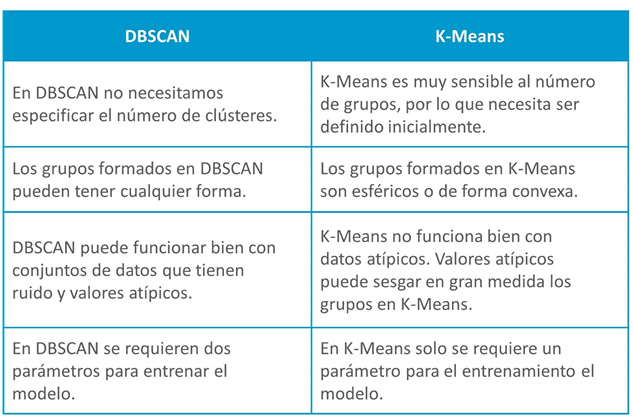
\includegraphics[width=0.85\linewidth]{imagenes/dbscan-kmeans.png}
    \label{fig:dbscan-kmeans}
\end{figure}


\section{Implementación de Python}
\subsection{KD-Tree}

Un KD-Tree (K-Dimensional Tree) es una estructura de datos en forma de árbol utilizada para organizar puntos en un espacio k-dimensional. Es particularmente útil para operaciones como la búsqueda de vecinos más cercanos y la agrupación de datos en algoritmos de aprendizaje automático y minería de datos.  Un KD-Tree es un árbol binario en el que cada nodo representa una partición de los puntos de datos en el espacio k-dimensional. Cada nodo tiene una «dimensión de corte» asociada y divide los puntos según su valor en esa dimensión

\subsection{R-Tree}
El R-Tree es una estructura de datos en forma de árbol utilizada para indexar información espacial o multidimensional. Es particularmente útil para realizar consultas espaciales eficientes, como encontrar todos los objetos dentro de una región dada. A diferencia de otros árboles, como el KD-Tree, el R-Tree está diseñado para manejar datos que no solo se representan como puntos, sino también como objetos de mayor dimensión (rectángulos, polígonos, etc.).

 
Un R-Tree está compuesto por nodos que contienen un número variable de entradas. Cada entrada en un nodo no hoja es un par formado por un identificador de nodo hijo y el MBR (Minimum Bounding Rectangle) de todos los objetos contenidos en ese nodo hijo.

\begin{itemize}
  \item Construimos un KD-Tree o un R-Tree a partir del conjunto de datos. Esto organiza los puntos de manera que las consultas espaciales sean más eficientes.
  \item Para cada punto en el conjunto de datos, en lugar de calcular la distancia a todos los otros puntos, utilizamos el árbol generado por el KD-Tree o el R-Tree para encontrar rápidamente todos los puntos dentro del radio \texttt{eps}.
  \item El KD-Tree y R-Tree permiten búsquedas eficientes en el espacio, lo que reduce el número de comparaciones y, por lo tanto, acelera el proceso de encontrar vecinos.
  \item Una vez que tenemos los vecinos, el algoritmo DBSCAN puede clasificar el punto actual como parte de un clúster, expandir el clúster o marcar el punto como ruido, según corresponda.
\end{itemize}


\begin{figure}[ht]
    \centering
    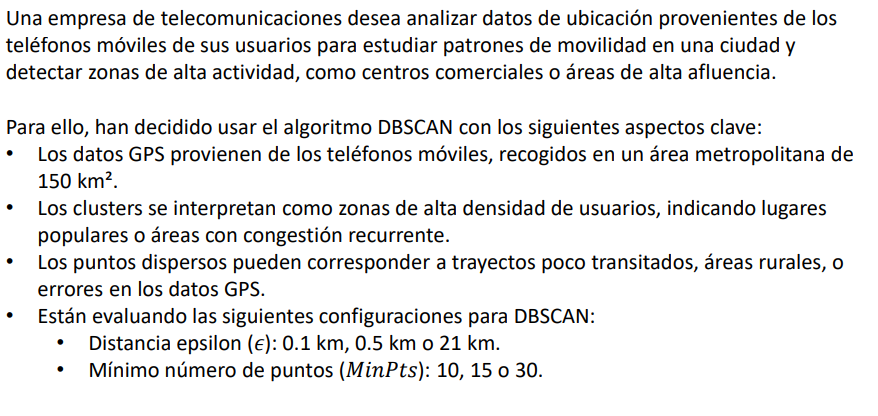
\includegraphics[width=0.85\linewidth]{imagenes/examen-dbscan1.png}
    \label{fig:examen-dbscan1}
\end{figure}


\begin{figure}[t]
    \centering
    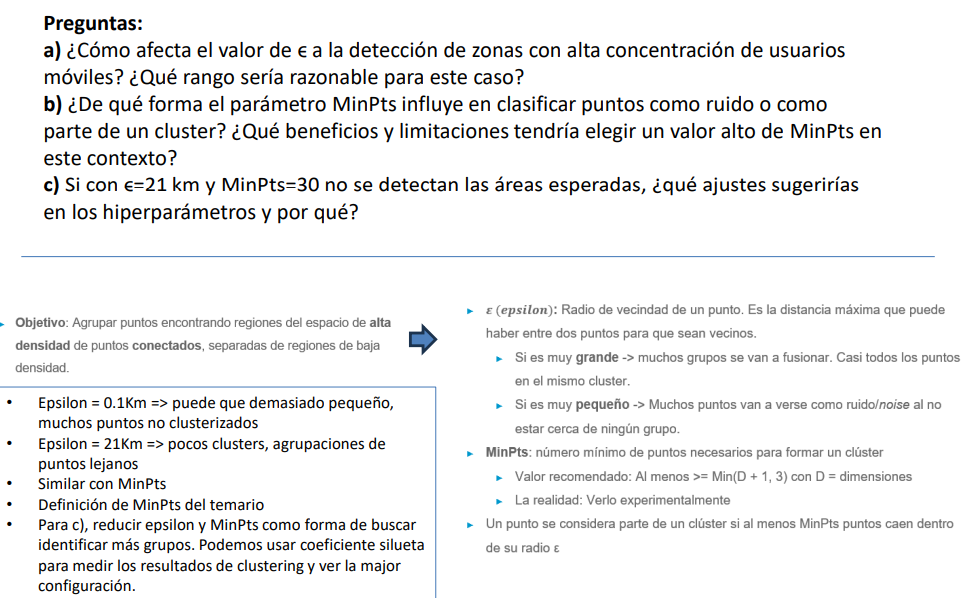
\includegraphics[width=0.85\linewidth]{imagenes/examen-dbscan2.png}
    \label{fig:examen-dbscan2}
\end{figure}